\documentclass{article}

\usepackage{amsmath}
\usepackage{fancyhdr}
\usepackage{graphicx}
\usepackage{hyperref}

\setcounter{secnumdepth}{0}

\pagestyle{fancy}
\lhead{}
\rhead{Universidad Católica de Córdoba}

\graphicspath{ {./images/} }

\renewcommand{\figurename}{Fig.}

\title{Estadística y Probabilidad (TICs)}
\author{Ivan L. Nuñez}
\date{}

\begin{document}

\begin{titlepage}
  \maketitle
  \thispagestyle{empty}
\end{titlepage}

\newpage
\renewcommand{\contentsname}{Índice}
\tableofcontents

\newpage
\section{Introducción}
En la cátedra de las TICs de la asignatura Estadística y Probabilidad de la
Universidad Católica de Córdoba, se nos presentó una actividad practica que
consta de realizar tres ejercicios. La profesora a cargo de la materia Franca
Giannini Kurina, será quien realizará la evaluación de suficiencia del mismo.
El límite de entrega del presente fue pactado para el 11 de Mayo de 2020.

Para realizar el trabajo utilice como leguaje de programación principal
Python ya que tengo varios años de experiencia desarrollando software con el.
Es pandas la librería que me facilitó la manipulación y el análisis de datos,
que además cuenta con otras dependencias utilizadas para realizar esquemas y
graficos a partir de la información recolectada. Todo el código escrito se
encuentra a disposición de todos en el siguiente link de mi repositorio de
GitHub: \url{https://github.com/ivanln26/eyp}.

\newpage
\section{Ejercicio 1}
Trabajas para el canal estatal que está diagramando una programación particular
para recreación por las tardes. Entre las actividades que te toca desempeñar te
piden un análisis de los temas más escuchados durante el 2019 y para eso te
facilitan una base de datos con las 100 canciones más escuchados durante el
2019 en la aplicación Spotify. Te entregan la base de datos y debes responder a
los principales interrogantes que la gerencia de producción detalla a
continuación, en un informe de un mínimo de dos páginas y un máximo de cuatro.
Para ello se recomienda utilizar herramientas de la estadística descriptivas
(tablas de medidas resúmenes, tablas de contingencia y gráficos), y se puede
utilizar además modelos probabilísticos en caso de ser factible.

En el contexto de la pandemia COVID-19 desde el canal queremos brindar un
programa vespertino donde la recreación y la actualidad sean prioridad.
Entendemos que los datos recolectados por la empresa Spotify nos pueden orientar
a la selección de material para musicalización y al proceso creativo general,
por lo tanto, aprovechando sus habilidades en análisis de datos le pedimos que
realice un análisis, para el cual detallamos la información que deseamos obtener
del mismo.  

Para empezar, sería bueno saber cuales son los géneros musicales más escuchados.
De cada género, se pretende conocer el nivel de popularidad, positividad y cuan
bailables son. A su vez, sería bueno agrupar los temas por la energía que
transmiten bajo algún criterio estadístico, ya que de eso depende en que parte
del programa se incluirían estos temas incluido. También nos interesa obtener
información respecto a los artistas para saber cuales se escucharon más. Por
último nos gustaría tener una idea general del comportamiento de las variables
que caracterizan los tracks musicales y como se relacionan entre si.

Cualquier otra información que consideres relevante de seguro nos será de gran utilidad.

Suerte con el análisis.
\begin{flushright}
  Gerencia de producción de contenido, canal 10.
\end{flushright}

\newpage
\subsection{Desarrollo}
A partir de la información obtenida luego del procesamiento de los datos
aportados, se llevó a cabo el análisis detallado de cada una de las
características pedidas por la gerencia de producción de contenido del canal 10.
A continuación les brindare las siguientes conclusiones:

\subsubsection{Géneros Musicales}
Como podemos observar en la figura 1, se presentan las frecuencias de la
aparicion de los generos musicales dentro de la lista de las canciones mas
escuchadas del 2019, el que destaca sobre los demas es \textit{dance pop},
ademas de contar con una gran ventaja. Los otros que se encuentran en el podio
del top 3 son \textit{latin} y \textit{pop}, siendo segundo y tercero
respectivamente. Entre la seccion \textit{others} (otros), que ocupan una gran
cantidad del grafico, se encuentran generos como.

En las figuras 2, 3 y 4 se presentan todos los generos musicales agrupados por
una caracteristica en particular especificada en el titulo superior de cada una.

\begin{figure}[h]
  \centering
  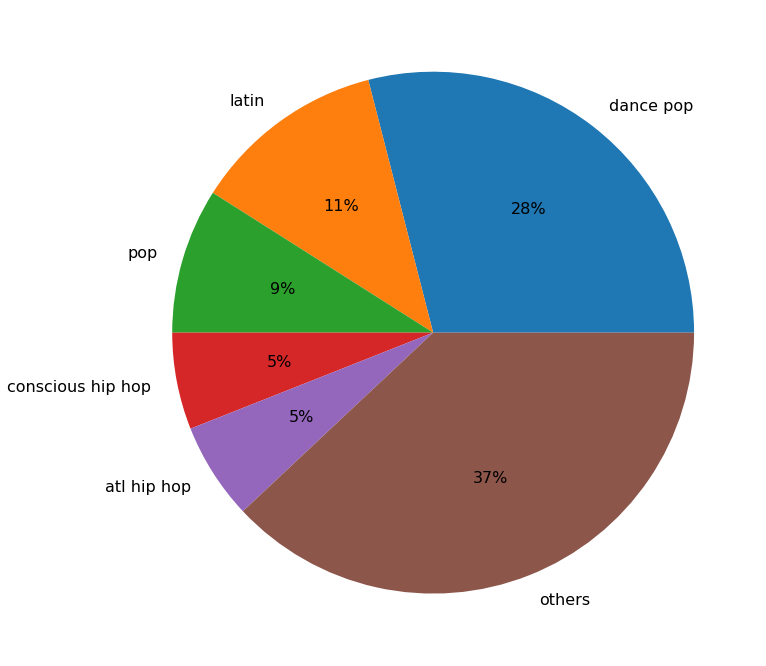
\includegraphics[scale=0.4]{a}
  \caption{gráfico de torta sobre géneros musicales.}
\end{figure}

\newpage
\subsubsection{Popularidad}

\begin{figure}[h]
  \centering
  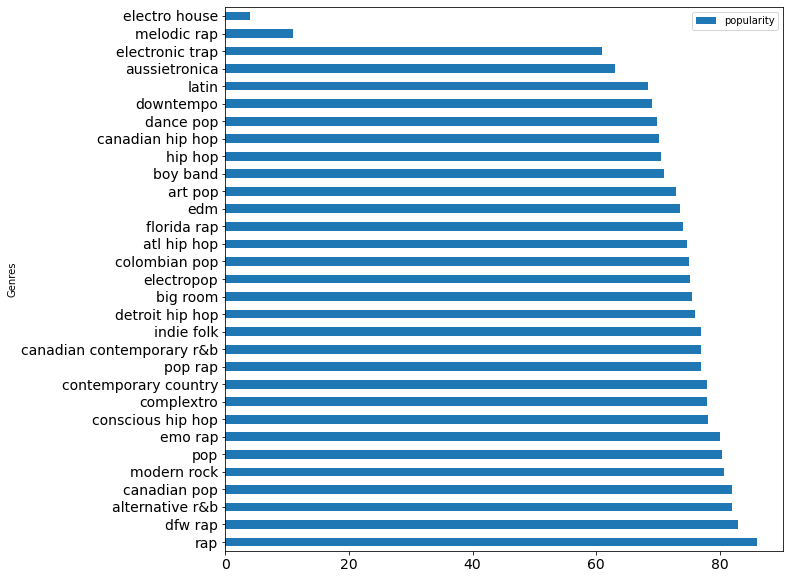
\includegraphics[scale=0.4]{b}
  \caption{gráfico de barras sobre popularidad agrupada por género.}
\end{figure}

\newpage
\subsubsection{Positividad}

\begin{figure}[h]
  \centering
  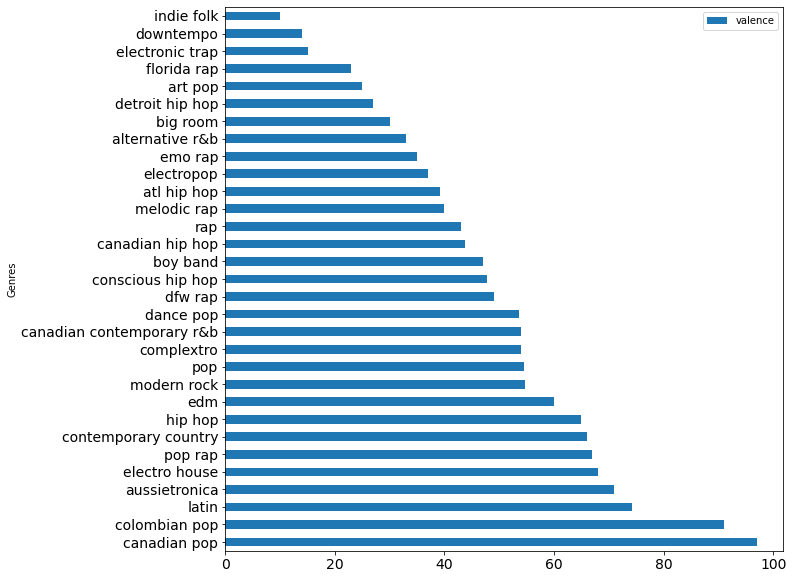
\includegraphics[scale=0.4]{c}
  \caption{gráfico de barras sobre positividad agrupada por género.}
\end{figure}

\newpage
\subsubsection{Bailabilidad}

\begin{figure}[h]
  \centering
  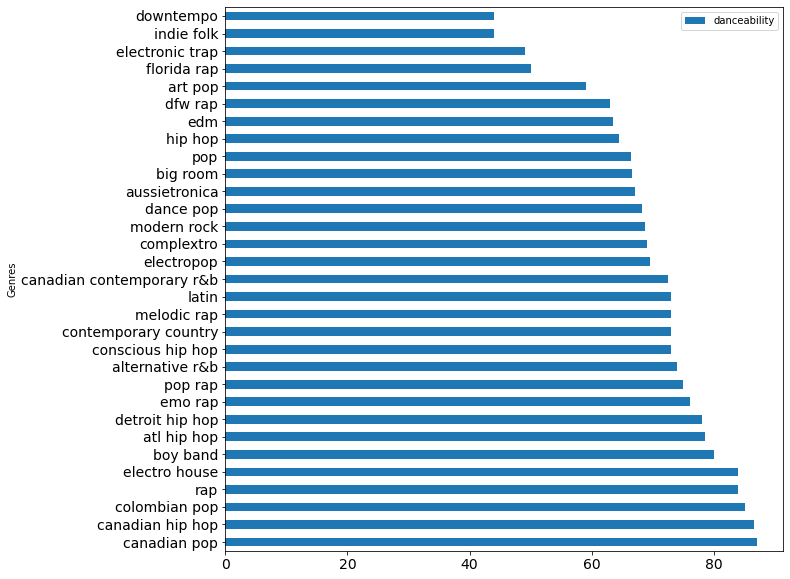
\includegraphics[scale=0.4]{d}
  \caption{gráfico de barras sobre bailabilidad agrupada por género.}
\end{figure}

\newpage
\subsubsection{Energía}
El criterio estadístico seleccionado para el agrupamiento de los temas por la
energía es la mediana. La medina nos permite conocer el punto que central que
existe en un rango, así como también obtener el promedio de la energía. En la
figura 5 se puede llegar a la conclusión de que el itervalo de energía que se
encuentra desde 55 hasta 85 es donde se produce la mayor concentración de
canciones.

\begin{figure}[h]
  \centering
  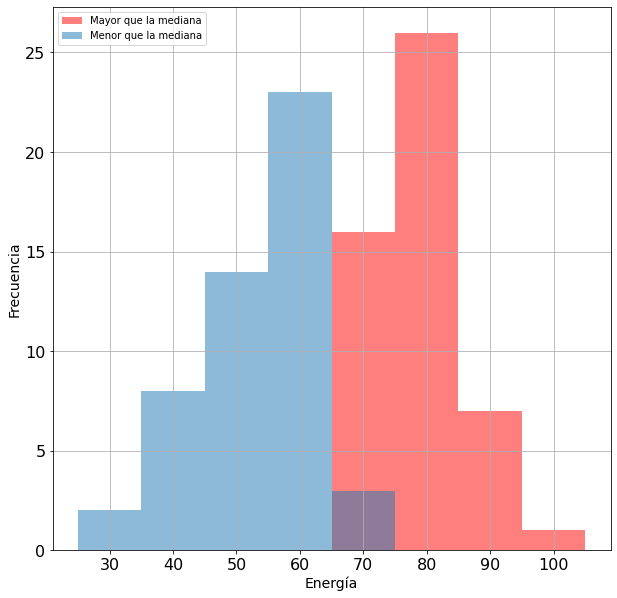
\includegraphics[scale=0.5]{e}
  \caption{histograma sobre la energía de los tracks.}
\end{figure}

\newpage
\subsubsection{Artistas}
En la figura 6, aparece el top 5 de los artistas más escuchados, y como podemos
oberervar, \textit{Kendrick Lamar} es el ganador y cuenta con 5 apariciones
dentro de la base de datos. Éste encuentra seguido por
\textit{Ed Sheeran, The Chainksmokers y Drake} quienes comparten el segundo
puesto y en donde cada uno cuenta con 4 registros.

\begin{figure}[h]
  \centering
  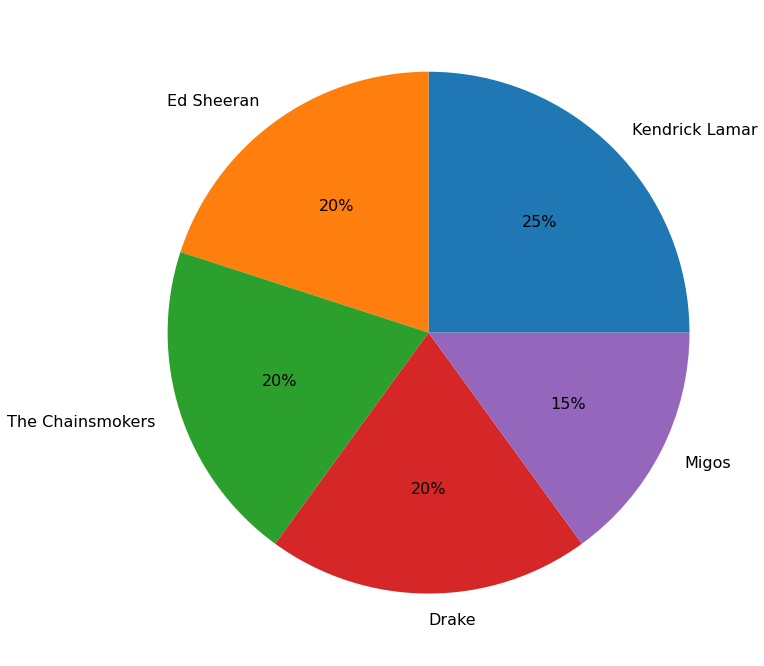
\includegraphics[scale=0.4]{f}
  \caption{gráfico de torta sobre los artistas más escuchasdos.}
\end{figure}

\newpage
\subsubsection{Comportamientos de las variables}
Los campos que seleccioné para el análisis del comportamiento de las variables
que caracterizan los tracks musicales son:
\textit{acústica, bpm, duración, fortaleza y cantidad de palabras}. Luego de
observar detenidamente estos campos de la figura 7, llegué a la conclusión de
que no existe alguna relación lo suficientemente estrecha para que genere algún
impacto sobre la selección de tracks.

\begin{figure}[h]
  \centering
  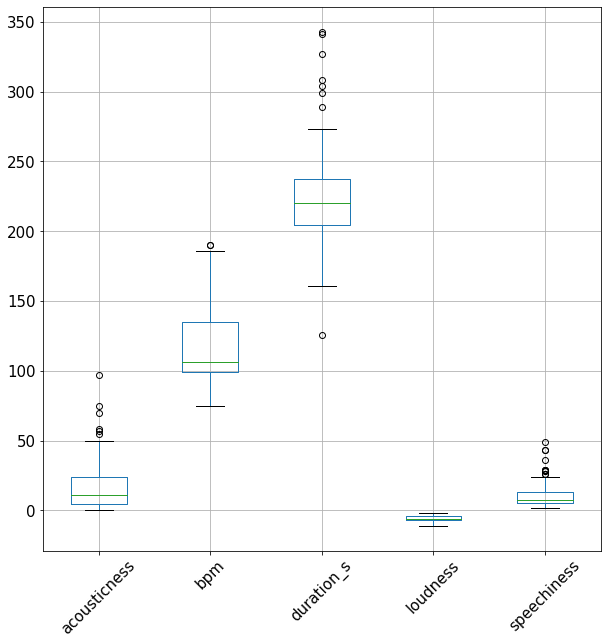
\includegraphics[scale=0.4]{g}
  \caption{gráfico de caja sobre las variables de los tracks.}
\end{figure}

\newpage
\section{Ejercicio 2}
Trabajando como gerente general y se encuentra a cargo un comité para evaluar
los desempeños de las distintas cadenas de la producción de la empresa. El
comité debe estar compuesto de compuesto de 10 personas debido a la cantidad de
tareas que implica la evaluación. Las personas que pueden integrar el comité son
aquellas en puestos gerenciales de la empresa en cada uno de los procesos. Los
gerentes son 16 hombres y 12 mujeres. La empresa tiene como política seleccionar
al azar los integrantes del comité, pero a la vez existen estándares de
evaluación externo que exigen que los puestos de auditoría y evaluación interna
sean equilibrados respecto al género. Responda:

\begin{enumerate}
  \item[a.] ¿Cuál es la probabilidad de que el comité esté compuesto de
    5 mujeres y 5 hombres?
  \item[b.] ¿Cuál es la probabilidad de que el comité esté compuesto de
    7 mujeres y 3 hombres?
  \item[c.] ¿Qué herramienta utilizó para responder a estos interrogantes?

  \item[\textbf{c}.] Para la resolución de este ejercicio, utilicé como
    herramienta la fórmula de distribución hipergeométrica. Siendo:
    \[ P(X = k) = \frac{\binom{K}{k} \binom{N - K}{n - k}}{\binom{N}{n}} \]
    Donde los coeficientes binomiales estan definidos como:
    \[ \binom{K}{k} = \frac{K!}{k! (K - k)!} \]
  \item[\textbf{a}.] \[
      P(X = 5) =
      \frac{\binom{16}{5} \binom{28 - 5}{10 - 5}}{\binom{28}{10}} = 0.263 \ldots
    \]
    \textbf{Rta}: la probabilidad de que el comité esté compuesto de 5 mujeres y
    5 hombres es aproximadamente de 0,263.
  \item[\textbf{b}.] \[
      P(X = 3) =
      \frac{\binom{16}{3} \binom{28 - 3}{10 - 3}}{\binom{28}{10}} = 0.033 \ldots
    \]
    \textbf{Rta}: la probabilidad de que el comité esté compuesto de 7 mujeres y
    3 hombres es aproximadamente de 0,033.
\end{enumerate}

\newpage
\section{Ejercicio 3}
Evaluando la rapidez de un servidor suponga que el tiempo de respuesta, X, en
cierta terminal de computadora en línea (en tiempo transcurrido entre el final
de la solicitud de un usuario y el comienzo de la respuesta del sistema a esa
solicitud) tiene distribución exponencial con tiempo de respuesta esperado igual
a 5''.

\begin{enumerate}
  \item[d.] La probabilidad de que el tiempo de respuesta sea, a lo sumo, 10''.
  \item[e.] La probabilidad de que el tiempo de respuesta esté entre 5'' y 10''.
\end{enumerate}

\subsection*{Datos}
\[ E(X) = \frac{1}{\lambda} = 5 \implies \lambda = 0.2 \]

\subsection*{Desarrollo}
\begin{enumerate}
  \item[d.]
    \[
      P(0 \leq X \leq 10) = \int_{0}^{10} \lambda e^{- \lambda x}\, \mathrm{d} x
    \]
    \[ \int_{0}^{10} 0.2 e^{- 0.2 x}\, \mathrm{d} x = 0.866466 \ldots \]
  \item[e.]
    \[
      P(5 \leq X \leq 10) = \int_{5}^{10} \lambda e^{- \lambda x}\, \mathrm{d} x
    \]
    \[ \int_{5}^{10} 0.2 e^{- 0.2 x}\, \mathrm{d} x = 0.23254 \ldots \]
\end{enumerate}

\end{document}
